% !TEX TS-program = pdflatex
% !TEX encoding = UTF-8 Unicode

% This is a simple template for a LaTeX document using the "article" class.
% See "book", "report", "letter" for other types of document.

\documentclass[11pt]{article} % use larger type; default would be 10pt

\usepackage[utf8]{inputenc} % set input encoding (not needed with XeLaTeX)

%%% Examples of Article customizations
% These packages are optional, depending whether you want the features they provide.
% See the LaTeX Companion or other references for full information.

%%% PAGE DIMENSIONS
\usepackage{geometry} % to change the page dimensions
\geometry{a4paper} % or letterpaper (US) or a5paper or....
% \geometry{margin=2in} % for example, change the margins to 2 inches all round
% \geometry{landscape} % set up the page for landscape
%   read geometry.pdf for detailed page layout information

\usepackage{graphicx} % support the \includegraphics command and options

% \usepackage[parfill]{parskip} % Activate to begin paragraphs with an empty line rather than an indent

%%% PACKAGES
\usepackage{booktabs} % for much better looking tables
\usepackage{array} % for better arrays (eg matrices) in maths
\usepackage{paralist} % very flexible & customisable lists (eg. enumerate/itemize, etc.)
\usepackage{verbatim} % adds environment for commenting out blocks of text & for better verbatim
\usepackage{subfig} % make it possible to include more than one captioned figure/table in a single float
% These packages are all incorporated in the memoir class to one degree or another...

%%% HEADERS & FOOTERS
\usepackage{fancyhdr} % This should be set AFTER setting up the page geometry
\pagestyle{fancy} % options: empty , plain , fancy
\renewcommand{\headrulewidth}{0pt} % customise the layout...
\lhead{}\chead{}\rhead{}
\lfoot{}\cfoot{\thepage}\rfoot{}

%%% SECTION TITLE APPEARANCE
\usepackage{sectsty}
\allsectionsfont{\sffamily\mdseries\upshape} % (See the fntguide.pdf for font help)
% (This matches ConTeXt defaults)

%%% ToC (table of contents) APPEARANCE
\usepackage[nottoc,notlof,notlot]{tocbibind} % Put the bibliography in the ToC
\usepackage[titles,subfigure]{tocloft} % Alter the style of the Table of Contents
\renewcommand{\cftsecfont}{\rmfamily\mdseries\upshape}
\renewcommand{\cftsecpagefont}{\rmfamily\mdseries\upshape} % No bold!

%%% END Article customizations

%%% The "real" document content comes below...

\title{Exploration of a Lock-Free Hash Table}
\author{Trevor Absher, Martin Dinkov}
%\date{} % Activate to display a given date or no date (if empty),
         % otherwise the current date is printed 

\begin{document}
\maketitle

\section{Abstract}

This paper expands upon the algorithm presented in \textit{Dynamic-Sized Nonblocking Hash Tables} by Liu et. al [1]. A specialization of their algorithm lies in "resizing in both directions: shrinking and growing." with the core of the algorithm being a "freezeable set abstraction, which greatly simplifies the task of moving elements among buckets during resize." [Liu et. al 2014]. Their algorithm is unique because previous attempts of a lock-free hash table (such as the variant by Shalev and Shavit [2]) did not support shrinking functionality. Furthermore, the freezable set abstraction in this paper expands on the normal operations of a set by adding a freeze method which prevents any thread from editing a given bucket while it is resized, simplifying the resize process [1].

We focus on the lock-free version of the hash table, using C++ to implement it. A minor difference lies in the fact that our implementation uses a Linked-List based set. The authors used a single flat array for its benefits regarding cache locality. However, an array-based implementation requires additional bookkeeping to avoid fragmentation. Our lock-free linked list Set implementation is derived from \textit{The Art of Multiprocessor Programming} by Herlihy and Shavit [3]. 

The idea of freezing the hash set relies on a resizing operation, dictated by a heuristic policy. The original paper does not cover any preferred heuristics. Thus, we compare the application of various commonly used policies. We also implement a transactional variant of a sequential hash table for the purpose of comparing it to our lock-free concurrent implementation. Each method of the sequential hash table is treated as a seperate transaction. Our testing for each solution is done across varying hardware architectures in order to explore the solution's portability.  

\section{Categories and Subject Descriptors}

D.1.3 [\textbf{Programming Techniques}]: Concurrent Programming -- \textit{Parallel Programming;} E.2 [\textbf{Data Storage Representations}]: Hash-table Representation

\section{Implementation}

In this section we will describe how we implemented each piece of Liu et. al's pseudocode while also implementing the code from Herlihy and Shavit.

\subsection{Freezable Set}

The Freezable Set object (FSet) was designed encapsulating the FSetOp object from the pseudocode and our own Set object. The FSet object contains only \textit{set} and \textit{ok} variables and an FSetOp struct. The \textit{ok} variable is a single bit representing whether or not the FSet is frozen. If \textit{ok} is set to false, then \textit{set} becomes immutable and no threads can add or remove an element. Threads can still check if an element is in the frozen set and retrieve it; which is important for the \textit{InitBucket} method of our HashTable, which will repopulate the current head node's buckets with the data from the previous head node.

\subsubsection{FSet Methods}

We next encapsulated the methods that affect an FSet object into the FSet class itself in order to simplify the calls. The \textit{HasMember} method takes in an integer and returns if it is found in the set or not. In our implementation, this calls the \textit{Set.contains()} method. The \textit{Invoke} method invokes either an add or remove operation based on the provided \textit{FSetOp} object. It first checks to make sure this operation has not already been completed and that it is a valid operation. This method calls both the \textit{Set.add()} and \textit{Set.remove()} methods depending on the \textit{op.type} variable; which is set to an enum of either \textbf{INSERT} or \textbf{REMOVE}. 

The \textit{Freeze} method is simple, yet crucial to the functionality of making the hash table lock free. We made no changes to the Freeze method provided by [1].

\subsubsection{FSetOp}

The FSetOp struct contains an enumeration with two values \textbf{INSERT} and \textbf{REMOVE} set to true and false respectively. The \textit{key} variable represents the integer that is going to be either added or removed. The \textit{done} bit is an atomic variable that represents if this specific add/remove operation has already been completed. The \textit{resp} bit is an atomic variable that represents if the operation was successful or not. The operation might fail if an add attempts to add a duplicate value, or if a remove attempts to remove a value that is not in the set. These variables are atomic to ensure all threads see the same statuses of these operations. The \textit{GetResponse} method retrieves the \textit{resp} variable of the object.

\subsection{Set}

The authors of [1] mention a set of integers, but do not go into detail as to how they implemented it. We decided on a Linked-List based Set class to represent the integer set of the FSet object. It is based off the Lock-Free version of the Set object given in \textit{The Art of Multiprocessor Programming} [3]. We made a slight modification to their Set object by adding a \textit{size} variable, which represents the size of each bucket. This variable is necessary as this is how our heuristic policies dictate when the buckets need to be resized. Initially, we made the size of the buckets 1000, with an estimate of 500,000 operations per test case. This Set class is made up of Node objects, also found in [3]. The only other change we make to the code provided by Herlihy and Shavit [3] is removing the \textit{key} variable from the Node class. Since we are using integers for the values we can simply sort the table on them, so we do not need a hash key. The Window object from [3] is also included for usage in traversing the list. 

\subsubsection{Set Methods}

All methods of our Set object are the same as those provided by [3], with an additional method \textit{Union}. A union operation is specified in the \textit{Invoke} method of [1] but in order to get the proper functionality we needed to abstract it into a method. It takes in a Set object and merges it with the Set object that called the method, returning the Set with all the data from both.


\subsection{Hash Table}

Next, we will go into details of how we implemented the Hash Node (HNode) object from [1]. We created a HashTable class with an HNode struct and encapsulated all the methods that operate on HNodes into the HashTable class. 

\subsubsection{Hash Table Methods}

The Hash Table has three public methods: \textit{Insert}, \textit{Remove}, and \textit{Contains}, all specified in [1]. There were no differences in our methods other than in \textit{Contains} where we made sure to atomically load the head node and the exact specifications of the heuristic-policy in \textit{Insert} and \textit{Remove}. Since [1] did not specify a heuristic policy there was no way we could implement theirs; in addition to us often changing the policy so we could experiment with which one performed the best.

The Hash Table also has three private methods and one private variable. The \textit{m\_head} variable is a pointer to an HNode object that is currently the head of the Hash Table. This variable is atomic, and all operations will be performed on the HNode that is the head of the Hash Table. Again, the only difference between our implementations was that we began by atomically loading the head node, which is never explicitly stated in the pseudocode provided by [1].


The \textit{Resize} method operates exactly as it does in the provided pseudocode from [1]. The Compare and Set call is done by making the head node atomic and then calling \textit{compare\_exchange\_strong}. The \textit{InitBucket} method also operates the same as in [1] with only a few differences to point out. The Set object initialized in this method is of our Set class implemented with the pseudocode from [3] and the Union performed on line 48 of the Lock-Free method of [1] is done using the \textit{Union} method of Set. Finally, the Compare and Set is done using a call to \textit{compare\_exchange\_strong} to put it into the HNode atomically since the buckets are also atomic. 

\subsubsection{HNode}

The HNode struct contains an array of atomic buckets in the form of FSet objects; denoted as \textit{buckets}. In order to determine which bucket a value goes into, we use the simple formula specified in [1]: index = k \textbf{mod} size. The \textit{size} variable denotes how many buckets there currently are in the given HNode. The \textit{pred} variable is of type HNode and points to the previous HNode in the Hash Table. This HNode will be either half or twice the size of the current HNode, depending on what resize operation was called to change it.

\section{Concurrency}

In this section we will discuss how the algorithm we implemented meets concurrency requirements.

\subsection{Progress Guarantees}

Our algorithm does not use any locks. All finalized changes done to either the head node or its buckets are done using the \textit{compare\_exchange\_strong} method, which is a version of the well-known Compare and Set method. If a thread fails to successfully update a value due to failing this \textit{compare\_exchange\_strong} call, it is likely due to the fact that the value it expected to be there was not, and thus the thread did not update the value to what it intended. This would only occur if the value had changed due to another thread coming in slightly before the first thread and changing the value. However, this means the second thread did successfully update the value. The first thread will try again to update the value (due to the \textit{resp} variable) but it may never succeed due to the same problem. If this same problem is occurring over and over, we know that the other threads are succesfully completing their operations. Since at least one thread can be guaranteed to successfully complete their operations and update the value, our algorithm is lock-free and thus is guaranteed to make progress. Even if a thread crashes during the \textit{Freeze} method and leaves the Set immutable without properly creating a new head node, the next FSetOp to attempt to insert or remove a value will fix this. The insert or remove will fail but the check for the heuristic policy will still trigger and this thread will then resize the Hash Table.

\subsection{Correctness Conditions}

All changes performed by inserts and removes will be performed only on the head node, and only on buckets. Both the head node and its buckets are atomic variables, which are guaranteed to only be edited by one thread at a time, and all threads will read the same value when reading an atomic variable. Since all updates to the head node and its buckets are done using  \textit{compare\_exchange\_strong}, we know that no threads will overwrite each other. The official updates to head and its buckets linearize at this method call, while the minor updates such as the insert, remove, and contains calls linearize when the \textit{op.done} variable is set to true. All the values for each slot in the sets of the buckets are also loaded atomically, so we know that we will receive the correct value when it is loaded. The \textit{Freeze} method also guarantees that no inserts or removes are lost during the time it takes a thread to successfully resize the Hash Table.


\subsection{Synchronization Techniques}

The main synchronization techniques used in this algorithm is the use of atomic variables and the \textit{compare\_exchange\_strong} method. The atomic variables ensure that every read to these variables will be synchronized so that every thread sees the same value at the same time. The \textit{compare\_exchange\_strong} method allows us to ensure only one thread will update the head node or its buckets at a time, protecting us from values getting incorrectly overwritten or certain calls returning invalid responses. However, the key synchronization technique in this algorithm is the \textit{Freeze} method. The \textit{ok} bit getting set to false stops every thread from editing the data of that HNode until the resize is complete. While this does interrupt progress for a time, this ensures that no data is lost while we switch the \textit{m\_head} variable to a new HNode. If \textit{Freeze} were not called, every insert and remove performed after the first line of \textit{Resize}, where we atomically load the current value of the head, would be lost.

\subsection{Transactional Implementation Using STM}

Software Transactional Memory (STM) libraries allow atomicity to be implemented in software for a set of operations, known as a transaction. Each transaction must be entirely executed or not at all. Such behavior requires rewinding functionality that allows all the progress made by a transaction up to a certain point to be undone if another transaction has overwritten data shared between the two transactions. Rewinding a transaction can introduce additional overhead that is not present within other methodologies. Nevertheless, if a transaction is being rewound, it is due to another transaction making progress.

\subsubsection{Sequential Hash Table}

STM allows for a sequential implementation of a data structure to be made concurrent by defining its operations as transactions. In fact, the implementation must be sequential because the STL atomic operations fail to compile if they are defined within a GCC STM transaction. This section covers the implementation of the sequential hash table, which mimics the lock-free version but without the thread-safety functionality.

Two different implementations for the hash table bins are explored. One implementation (Sequential::Set class) utilizes a binary search tree for its quick logarithmic-time search functionality. The other implementation utilizes a linked-list (Sequential::List) for its ability to be easily split into two lists or combined with another list into a single one. The benefit of using the List class for the bins is only apparent if the hash table supports proper resizing hierarchy. Without proper resizing, the bins may grow too large and in which case the linear search time of the List make it inferior to the Set.

In addition to the traditional Insert, Remove, and Contains operations, the Set and List classes also include a Union and IntersectRemainder operations. Just like in the lock-free hash table, they are used when resizing the number of bins. Union combines two bins together while IntersectRemainder splits a bin into two based on the remainder value when dividing each element. These operations are simplified in the List implementation because:

\begin{itemize}
	\item An existing list can be recycled
	\begin{itemize}
		\item During a Union, the elements of the shorter List are inserted into the longer list.
	\end{itemize}
	\item Since both Lists are always sorted, each of these operations require a single traversal through each List resulting in an O(m+n) complexity.
	\begin{itemize}
		\item On the other hand, the time complexity of equivalent calls in Set is O(m * (n * log(n))) since each the tree has to be re-traversed for each Insert.
	\end{itemize}
\end{itemize}

A set of verification tests are included in Tests.h that check the correctness of the Set and List classes. This code can be triggered by running the SequentialHashTable executable with an invalid set of parameters.

The InsRem-50-64K data set is used to compare the different variants of the Sequential::HashTable since it is the most stressful. The single-threaded results are shown below, which confirm the differences between the Set and List implementations.

\begin{itemize}
	\item Sequential::Set is used for bin implementation and resizing is DISABLED.
	\begin{itemize}
    		\item 195ms
	\end{itemize}
	\item Sequential::Set is used for bin implementation and resizing is ENABLED.
	\begin{itemize}
		\item 118ms
	\end{itemize}
	\item Sequential::List is used for bin implementation and resizing is DISABLED.
	\begin{itemize}
		\item 6494ms
	\end{itemize}
	\item Sequential::List is used for bin implementation and resizing is ENABLED.
	\begin{itemize}
		\item 100ms
	\end{itemize}
\end{itemize}

From here on, Sequential::List is used with resizing enabled. Various resize hierarchies are explored in this implementation, as for the lock-free hash table. Resizing based on the cumulative number of entries in the hash table again proves to be more efficient than resizing based on the size of individual bins. Resizing based on individual bins can lead to the number of bins constantly fluctuating if one bin has a lot of entries and another bin has very few. The lower threshold was chosen to be equal to numBins, since the optimal upper threshold showed to be 4 * numBins. Having thresholds that are > 2 times apart eliminates the possibility of resizing twice in two consecutive operations.

\begin{itemize}
	\item Resizing based on bin size. This can be enabled by changing the “\#if 0” occurrences in Sequential::HashTable to “\#if 1”
	\begin{itemize}
    		\item 170ms
	\end{itemize}
	\item Resizing based on cumulative number of entries in hash table. Upper threshold is set to 2 * numBins. Lower threshold is set to numBins.
	\begin{itemize}
		\item 123ms
	\end{itemize}
	\item Resizing based on cumulative number of entries in hash table. Upper threshold is set to 4 * numBins. Lower threshold is set to numBins.
	\begin{itemize}
		\item 100ms
	\end{itemize}
	\item Resizing based on cumulative number of entries in hash table. Upper threshold is set to 8 * numBins. Lower threshold is set to numBins.
	\begin{itemize}
		\item 109ms
	\end{itemize}
\end{itemize}

\subsubsection{One Operation Per Transaction}

The GCC transactional memory library is used in this implementation instead of RSTM because GCC is more commonly used and thus more likely to be streamlined. Also, the GCC transactions are implemented at the compiler level and are thus likely to be more efficient. Initially, each Sequential::HashTable operation is wrapped in its own transaction using the \_\_transaction\_atomic compiler directive. This compiler directive does not allow the compiler to insert locks, unlike the \_\_transaction\_relaxed directive [4]. SuperMalloc is used in this implementation as well in order to provide thread-safe memory allocations and deallocations. Introducing SuperMalloc did not create a noticeable change in performance.

The table below shows the results of having a single operation per each atomic transaction. The runtime of the single threaded test cases have likely increased due to the overhead of preparing and submitting the transactions. The runtime becomes progressively worse with each additional thread since there are various possibilities for collisions throughout every function. Contains is the only exception, hence why it shows the best performance.

\bigskip
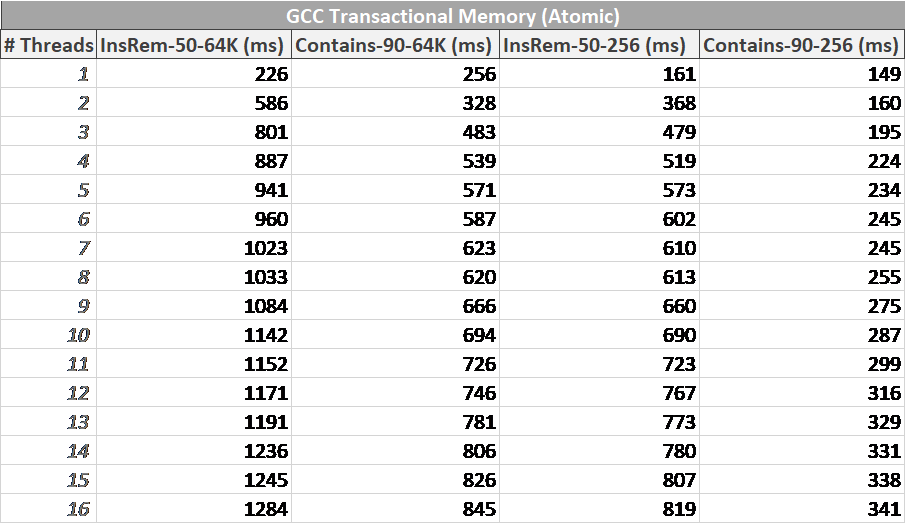
\includegraphics[width=0.5\linewidth]{Table1.png}
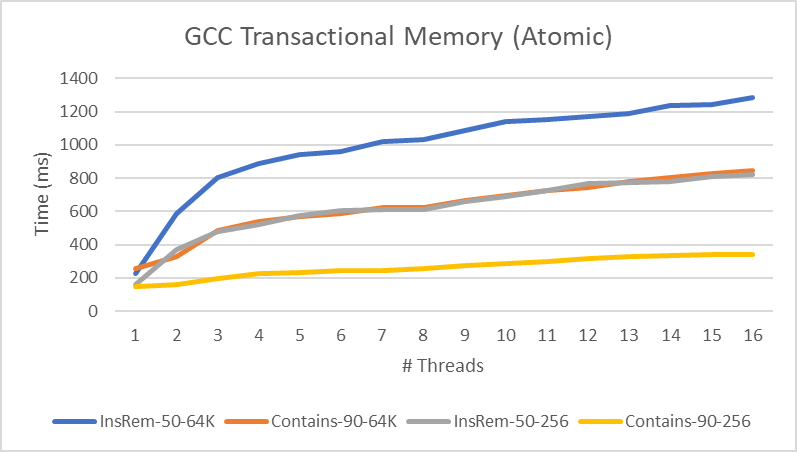
\includegraphics[width=0.5\linewidth]{Graph1.png}

\subsubsection{Multiple Operations Per Transaction}

Packing multiple operations within a transaction proves to be more efficient for this kind of hash table. Having less transactions overall leads to less overhead dedicated to handling and submitting the transactions. This performance gain is directly reflected in the single-threaded case. However, having longer transactions leads to longer rewind procedures. This is likely why the rate of change drastically increases beyond 8 threads in the charts below, when collisions become much more likely.

The graph below shows the results from having two operations per transaction. This is significantly more performant than having a single operation per thread, since the gain of having to do bookkeeping for less transactions outweighs the loss of the transactions being longer. With more threads, this case is likely to become less performant than having a single operation per transaction.

\bigskip
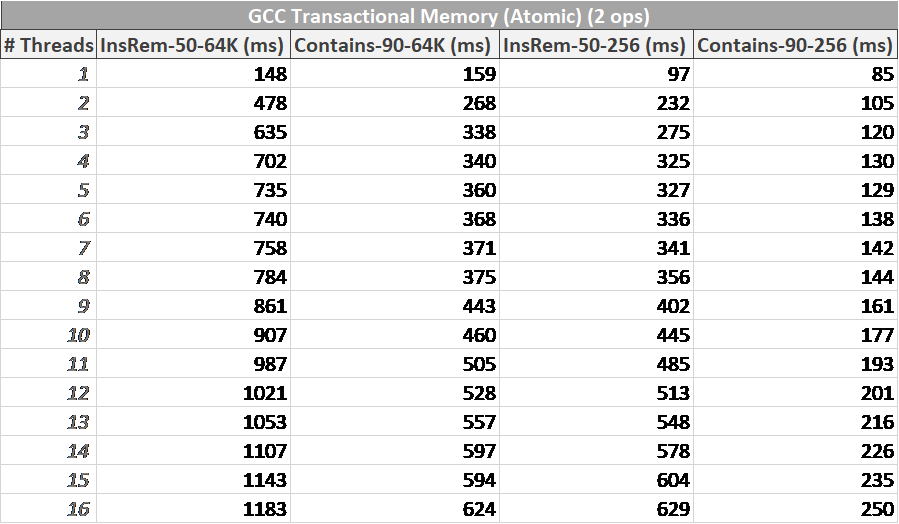
\includegraphics[width=0.5\linewidth]{Table2.png}
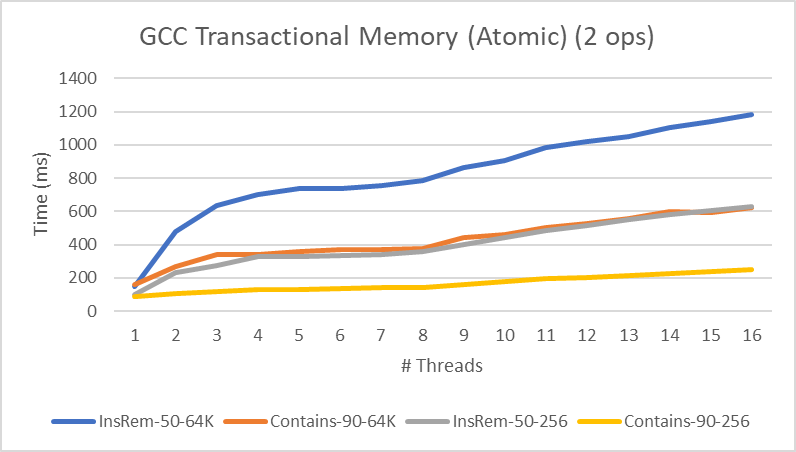
\includegraphics[width=0.5\linewidth]{Graph2.png}

The graph below shows the results from having four operations per transaction. It is more efficient than the either of two previous cases at lower number of threads. However, at higher number of threads it becomes no better than having two operations per transaction.

\bigskip
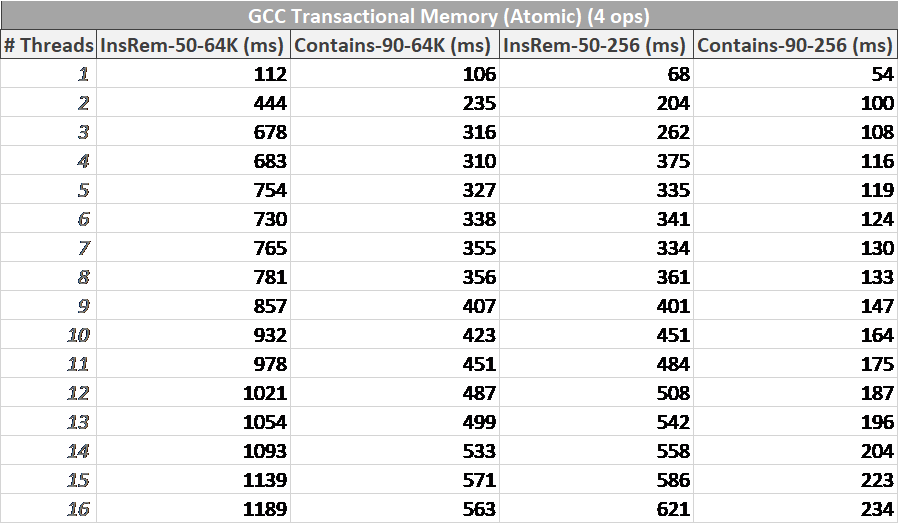
\includegraphics[width=0.5\linewidth]{Table3.png}
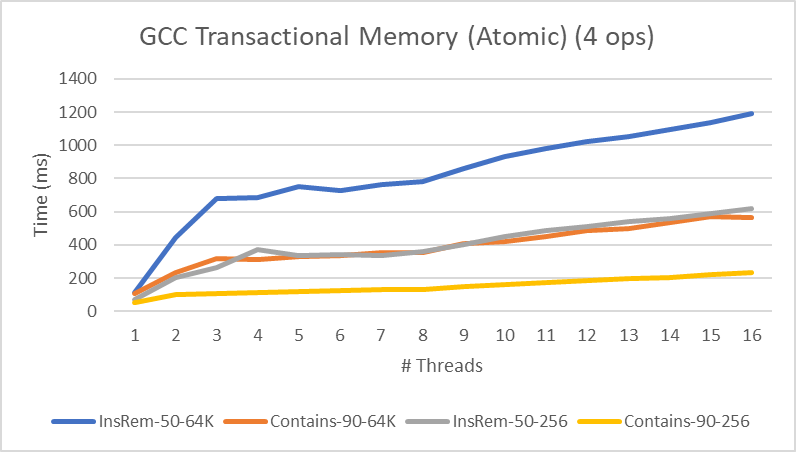
\includegraphics[width=0.5\linewidth]{Graph3.png}

\subsubsection{Improvement Attempts}

This section covers several attempts to improve upon the STM implementation of the hash table. The only one that proves to be effective is to use coarse-grained locks instead of transactions for this kind of data structure.

\subsubsection{Relaxed Transactions}

Having relaxed transaction instead of atomic ones allows GCC to determine if using locks for some cases can be more efficient than atomicity. Atomicity can become too convoluted to implement in some cases [4]. The data below show the results of using relaxed transactions for the case where a transaction includes only a single operation. It seems no different from the case where the transactions are strictly atomic. The results from having relaxed transactions for the cases where a transaction encompasses multiple operations are also like the ones with strictly atomic transactions.

\bigskip
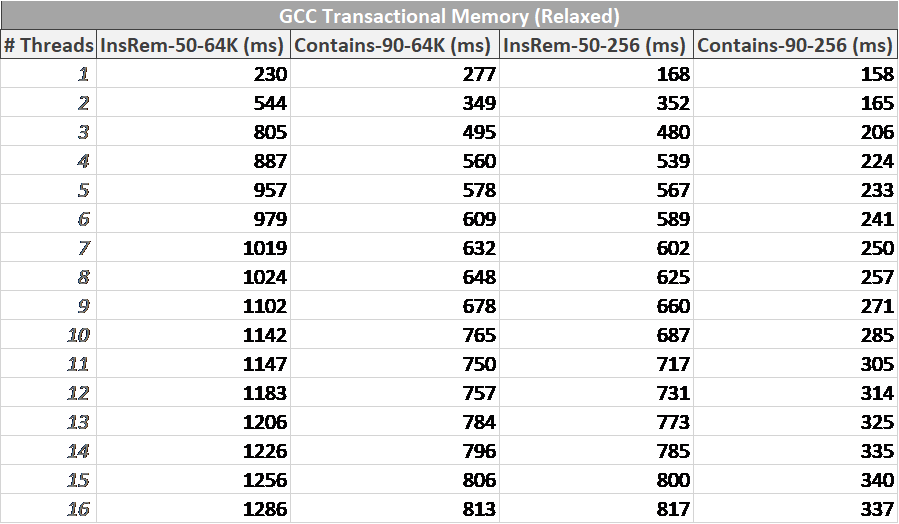
\includegraphics[width=0.5\linewidth]{Table4.png}
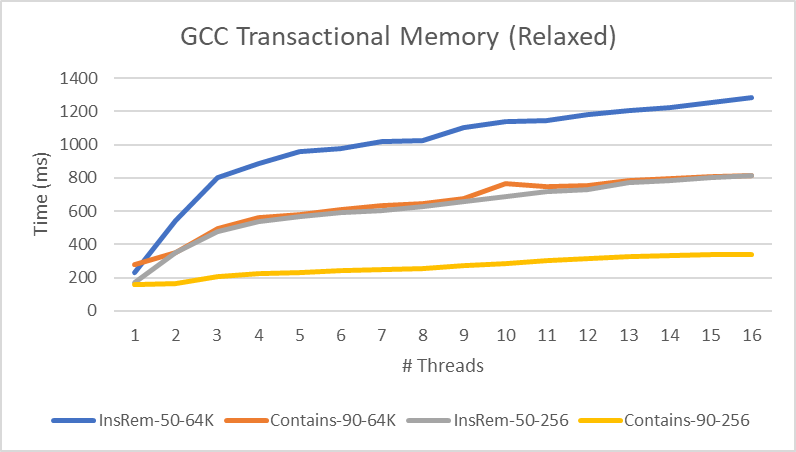
\includegraphics[width=0.5\linewidth]{Graph4.png}

\subsubsection{Replacing Transactions with Locks}

Using locks (via std::mutex) instead of transactions showed approximately 20\% higher performance. Mutexes synchronize the operations, but collisions are eliminated and thus rewinds are no longer necessary. The data below shows the results from wrapping each operation in a mutex. If multiple operations are wrapped, then the performance is likely to be even better since there will be less contention points.

\bigskip
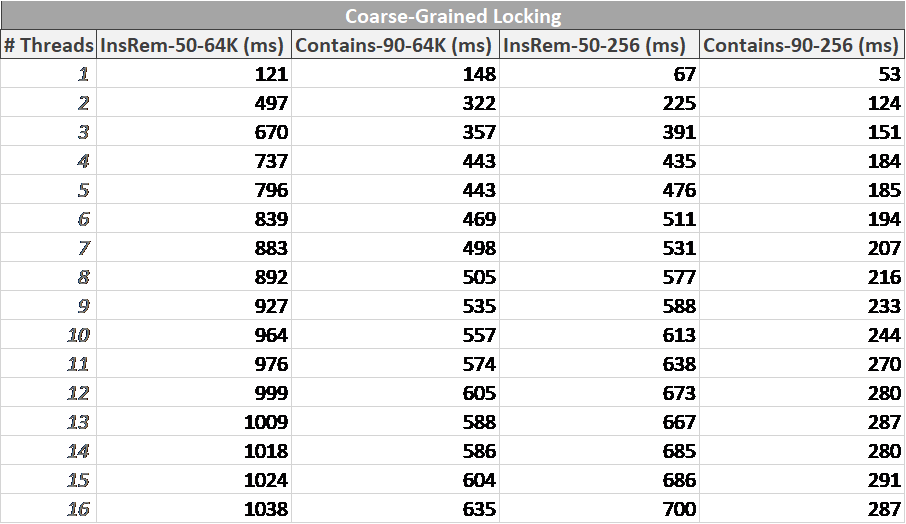
\includegraphics[width=0.5\linewidth]{Table5.png}
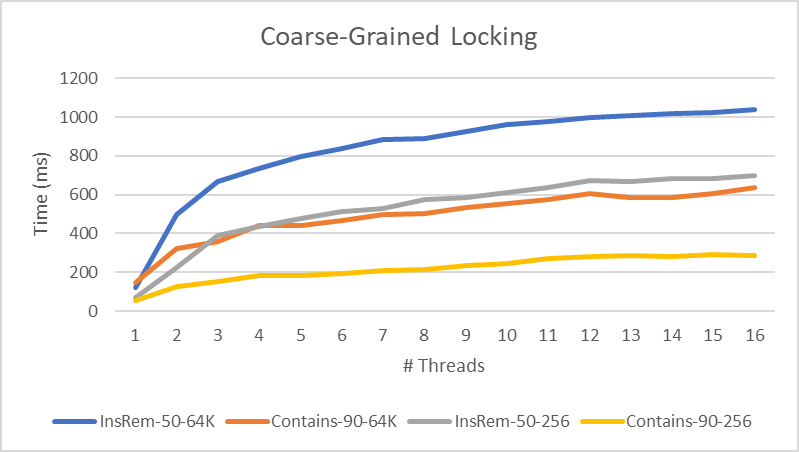
\includegraphics[width=0.5\linewidth]{Graph5.png}

\subsubsection{Offsetting the Transactions}

The synchronize keyword in GCC allows a block of code to always executed sequentially. Under the hood, this is likely implemented using locks and requires that the transactions be relaxed. Wrapping various points of the code to offset the transactions and reduce the number of collisions leads to an increased overall execution time. The collisions likely still occur, and additional overhead is introduced by serializing parts of the code.

\subsubsection{Comparison to Lock-Free Implementation}

The STM implementation of the Hash Table does not scale well with additional threads, in contrast to the lock-free implementation. The two implementations have comparable performance only when using two threads are being executed. However, the STM implementation is significantly simpler to apply to a sequential data-structure.

\section{Performance Evaluation}

In this section we will compare the performance of our implementation of the algorithm versus the official algorithm provided by Liu et. al in [1]. We also will compare the performance of our different heuristic policies. Finally, we measure the performance differences between our initial implementation in a concurrent data structure and our final implementation where we converted it to a transactional data structure.

\section{Conclusion}

In this paper, we introduced our own implementation of the Lock-Free Dynamic-Sized Nonblocking Hash Tables created by Liu et. al in [1]. Our implementation differed from theirs in a few ways. First, our Set object was a linked list as opposed to an array. While the array has superior locality of memory, the authors of [1] did not provide information as to how they implemented it. Next, we implemented a size variable and a few threshold variables. While these were not explicitly stated by the authors of [1], it is more than likely they had something similar in place otherwise they would not have been able to have anything to determine their heuristic policy off of. Our size variable tracked the current size of each bucket, while the lower threshold was the bound for shrinking the Hash Table, and the upper threshold was the bound for growing the Hash Table. The max size variable provided a maximum number of buckets so that the memory would not grow exponentially if threads continually needed to make buckets by adding similarly hashed values. Our final difference was our heuristic policy. Again, this difference was due to the authors of [1] not stating exactly what heuristic policy they used, as this was not the goal of their paper. We first implemented a simple policy, growing when the current bucket was too big, and shrinking when it was too small. Next, we tried what the authors suggested and grew when the current bucket was too big and shrunk when a random sample of buckets were all too small. Finally, the last policy we tried (which also performed the best) was to resize based on the cumulative size of all the entries in all buckets. 

Re-implementing Liu et. al's data structure was not without its challenges. Converting their pseudocode to functional C++ code was often difficult, especially with certain operations that were not explicitly coding techniques, such as the union operation found in the pseudocode for the FSet object. Implementing the parts of the data structure not described by the authors was also troublesome. Coming up with our own heuristic policies to resize the hash table on took some time and we had to entirely change the Set from operating on an array to operating on a linked list, which involved creating a whole new class with all of its own methods. Using the size variable of each bucket also proved challenging. Without using a Descriptor object, the size variable was not perfectly thread safe. Retrieving the size variable at any given time may not have been the true correct value of the size by the time it was used. However, implementing a Descriptor object would have complicated the data structure even more, so this was determined to be acceptable. To make up for this, the maximum size of each bucket was not enforced, but a suggestion. The hash table would be resized when a bucket grew close to its maximum size, but if threads attempted to add values to it before this size was properly read by the resize operation, the values would still be added to the bucket and would not be lost. 

This data structure provides a lot of new advantages to existing alternatives. The biggest its dynamic property; being able to grow and shrink while previous hash table implementations were only able to grow. In an environment with limited memory this data structure is far optimal to its alternatives due to this key feature. It also allows keys to be moved among buckets during a resize operation which previous data structures have not done. Doing this during the resize allows this implementation to avoid sacrificing throughput or progress. Also, the buckets are unbounded and no assumption is made about the size of memory, which allows this data structure to be more flexible in its applications onto larger datasets. While the inner mechanisms of this data structure can be complicated, as there are four encapsulating layers of objects; once it has been successfully implemented the advantages of it far outweigh this.



\nocite{*}
\bibliography{bibliography}
\bibliographystyle{IEEEtr}


\end{document}
